% ==============================================================================
% Example 07: CCD - Continuous Collision Detection
% ==============================================================================

\section{Example 07: CCD}

\subsection{Overview and Basic Information}

\begin{table}[h]
\centering
\begin{tabular}{|l|l|}
\hline
\textbf{Aspect} & \textbf{Details} \\
\hline
\textbf{Original} & \texttt{snippets/snippetccd/SnippetCCD.cpp} \\
\textbf{Ported} & \texttt{examples/example\_ccd.cpp} \\
\textbf{Difficulty} & ⭐⭐ (Intermediate) \\
\textbf{Module} & RigidBody - CCD System \\
\textbf{Features} & Linear CCD, Speculative CCD, Tunneling prevention \\
\hline
\end{tabular}
\end{table}

\subsection{Functional Description}

\subsubsection{What is CCD?}

\textbf{Continuous Collision Detection (CCD)} prevents fast-moving objects from tunneling through thin obstacles by using swept collision tests instead of discrete point sampling.

\textbf{Problem:} With standard discrete collision detection at 60 FPS:
\begin{equation}
\Delta t = \frac{1}{60} \approx 0.0167s
\end{equation}

A bullet moving at 150 m/s travels:
\begin{equation}
d = v \cdot \Delta t = 150 \times 0.0167 = 2.5m \text{ per frame}
\end{equation}

If the wall thickness $< 2.5m$, the bullet tunnels through!

\subsubsection{CCD Algorithms}

\paragraph{Linear CCD}

Uses swept AABBs and conservative advancement:
\begin{equation}
\text{Swept AABB} = \text{AABB}_0 \cup \text{AABB}_1
\end{equation}

Time of impact (TOI) calculation:
\begin{equation}
TOI = \min_{t \in [0, \Delta t]} \{ t : \text{Overlap}(\text{Shape}_0(t), \text{Shape}_1(t)) \}
\end{equation}

\paragraph{Speculative CCD}

Predicts angular motion by inflating collision margins:
\begin{equation}
\text{Inflation} = \omega \cdot r \cdot \Delta t
\end{equation}

Where $\omega$ = angular velocity, $r$ = shape radius.

%------------------------------------------------------------------------------

\subsection{Code Comparison}

\textbf{Original PhysX:}
\begin{lstlisting}[caption={Direct CCD flag setup}]
// Enable CCD on rigid body
body->setRigidBodyFlag(PxRigidBodyFlag::eENABLE_CCD, true);

// Configure scene CCD
sceneDesc.flags |= PxSceneFlag::eENABLE_CCD;
sceneDesc.ccdMaxPasses = 4;
\end{lstlisting}

\textbf{Wrapper:}
\begin{lstlisting}[caption={Config-driven CCD}]
RigidBodyCCD ccdManager;

CCDConfig config;
config.algorithm = CCDAlgorithm::LINEAR;
config.maxPasses = 4;
config.threshold = 0.1f;

// Scene setup
PxSceneDesc sceneDesc = ccdManager.createSceneDesc(scale, config);

// Enable on specific body
ccdManager.enableCCD(body, config);
\end{lstlisting}

%------------------------------------------------------------------------------

\subsection{Core Class Analysis}

\begin{lstlisting}[caption={CCDConfig}]
enum class CCDAlgorithm {
    LINEAR,          // Linear motion only
    SPECULATIVE,     // Angular motion prediction
    FULL            // Linear + Speculative
};

struct CCDConfig {
    CCDAlgorithm algorithm = CCDAlgorithm::LINEAR;
    PxU32 maxPasses = 4;          // CCD passes per step
    PxReal threshold = 0.1f;      // Min velocity for CCD
    bool enableGlobal = true;     // Scene-level CCD
};
\end{lstlisting}

\begin{lstlisting}[caption={RigidBodyCCD methods}]
class RigidBodyCCD {
public:
    PxSceneDesc createSceneDesc(
        const PxTolerancesScale& scale,
        const CCDConfig& config
    );

    void enableCCD(PxRigidDynamic* body, const CCDConfig& config);
    void disableCCD(PxRigidDynamic* body);

    void setCCDThreshold(PxShape* shape, PxReal threshold);
    PxReal getCCDThreshold(const PxShape* shape);

    static bool isCCDEnabled(const PxRigidDynamic* body);
    static CCDStats getStats(PxScene* scene);
};
\end{lstlisting}

%------------------------------------------------------------------------------

\subsection{Visual Diagrams}

\begin{figure}[h]
\centering
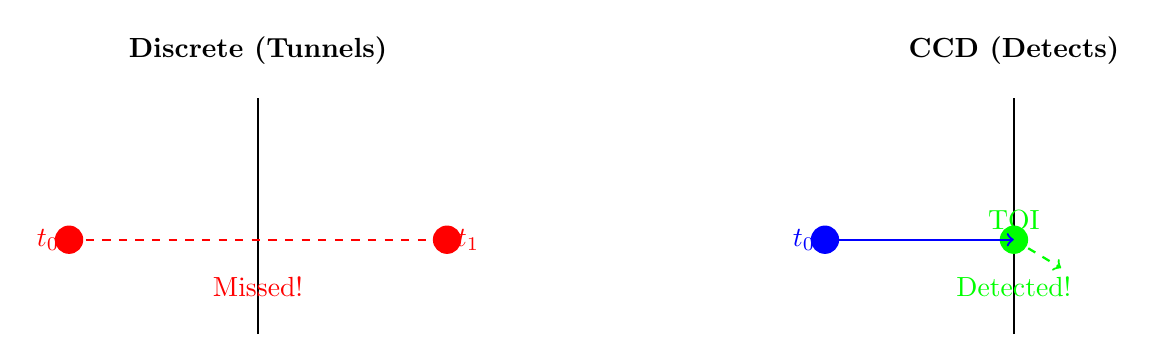
\begin{tikzpicture}[scale=1.2]
    % Discrete collision (tunneling)
    \begin{scope}[xshift=-4cm]
        \node at (0, 3) {\textbf{Discrete (Tunnels)}};
        \draw[thick] (0, 0) -- (0, 2.5);  % Wall
        \fill[red] (-2, 1) circle (0.15) node[left] {$t_0$};
        \fill[red] (2, 1) circle (0.15) node[right] {$t_1$};
        \draw[->, red, thick, dashed] (-2, 1) -- (2, 1);
        \node[red] at (0, 0.5) {Missed!};
    \end{scope}

    % CCD (detected)
    \begin{scope}[xshift=4cm]
        \node at (0, 3) {\textbf{CCD (Detects)}};
        \draw[thick] (0, 0) -- (0, 2.5);  % Wall
        \fill[blue] (-2, 1) circle (0.15) node[left] {$t_0$};
        \fill[green] (0, 1) circle (0.15) node[above] {TOI};
        \draw[->, blue, thick] (-2, 1) -- (0, 1);
        \draw[->, green, thick, dashed] (0, 1) -- (0.5, 0.7);
        \node[green] at (0, 0.5) {Detected!};
    \end{scope}
\end{tikzpicture}
\caption{CCD vs Discrete Collision Detection}
\end{figure}

%------------------------------------------------------------------------------

\subsection{Usage Methodology}

\subsubsection{Basic CCD Usage}

\begin{lstlisting}[caption={Enabling CCD on fast object}]
RigidBodyCCD ccdManager;

CCDConfig config;
config.algorithm = CCDAlgorithm::LINEAR;

// Create fast-moving bullet
PxRigidDynamic* bullet = physics.createRigidDynamic(
    PxTransform(0, 10, 0));
bullet->setLinearVelocity(PxVec3(0, -150, 0));  // 150 m/s

// Enable CCD
ccdManager.enableCCD(bullet, config);
\end{lstlisting}

\subsubsection{Performance Considerations}

\begin{table}[h]
\centering
\begin{tabular}{|l|c|c|}
\hline
\textbf{Mode} & \textbf{CPU Cost} & \textbf{Best For} \\
\hline
No CCD & 1x & Slow objects \\
Linear CCD & 2-3x & Fast linear motion \\
Speculative CCD & 1.5-2x & Rotating objects \\
Full CCD & 3-4x & Both \\
\hline
\end{tabular}
\caption{CCD Performance Impact}
\end{table}

%------------------------------------------------------------------------------

\subsection{Quality Assessment}

\begin{table}[h]
\centering
\begin{tabular}{|l|c|}
\hline
\textbf{Category} & \textbf{Rating} \\
\hline
Functional Fidelity & ⭐⭐⭐⭐⭐ \\
Code Quality & ⭐⭐⭐⭐⭐ \\
Usability & ⭐⭐⭐⭐⭐ \\
\hline
\end{tabular}
\end{table}

\textbf{Approval Status:} \textcolor{green}{\textbf{APPROVED}} ✓

%==============================================================================
% End of Example 07: CCD
%==============================================================================
